\documentclass[10pt,xcolor={usenames},fleqn,mathserif,serif]{beamer}

\hypersetup{pdfpagemode=FullScreen}

%% colors
\definecolor{bittersweet}{rgb}{1.0, 0.44, 0.37}
\definecolor{brilliantlavender}{rgb}{0.96, 0.73, 1.0}
\definecolor{antiquefuchsia}{rgb}{0.57, 0.36, 0.51}
\definecolor{violetw}{rgb}{0.93, 0.51, 0.93}
\definecolor{Veronica}{rgb}{0.63, 0.36, 0.94}
\definecolor{atomictangerine}{rgb}{1.0, 0.6, 0.4}
\definecolor{darkgray}{rgb}{0.66, 0.66, 0.66}
\definecolor{brightcerulean}{rgb}{0.11, 0.67, 0.84}
\definecolor{cadmiumorange}{rgb}{0.93, 0.53, 0.18}
\definecolor{ochre}{rgb}{0.8, 0.47, 0.13}
\definecolor{midnightblue}{rgb}{0.1, 0.1, 0.44}
\definecolor{lemon}{rgb}{1.0, 0.97, 0.0}
\definecolor{grey}{rgb}{0.7, 0.75, 0.71}
\definecolor{amber}{rgb}{1.0, 0.75, 0.0}
\definecolor{almond}{rgb}{0.94, 0.87, 0.8}
\definecolor{bf}{RGB}{88, 86, 88}
\definecolor{bb}{RGB}{177, 177, 177}


%%%%%%%%%%%%%%%%%%%%%%%%%%%%%%%%%%% importa pacchetti
\usepackage{usepkg}
%%%%%%%%%%%%%%%%%%%%%%%%%%%%%%%%%%% Funzioni generali
\usepackage{functions}
%http://tex.stackexchange.com/questions/246/when-should-i-use-input-vs-include
\newcommand{\setmuskip}[2]{#1=#2\relax} %%problem usinig mu with calc (req by mathtools) loaded
\usepackage{beamersetup}
\usepackage{sources}
%\usepackage{length}
%%%%%%%%%%%%%%%%%%%%%%%%%%%%%%%%%%% Funzioni per questo file main
\usepackage{mathOp}
\def\status{coazione}%ripeter
\def\keeptrying{coazione}
\usepackage{LocalF}
%%%%%%%%%%%%%%%%%%%%%%%%%%%%%%%%%

\title{Osservazione sistemi planetari extra-solari (Beamer)}

% A subtitle is optional and this may be deleted
\subtitle{Tecniche osservative sistemi planetari. Osservazione \ldots}

%\author{F.~Author\inst{1} \and S.~Another\inst{2}}
% - Give the names in the same order as the appear in the paper.
% - Use the \inst{?} command only if the authors have different
%   affiliation.

%\institute[Universities of Somewhere and Elsewhere] % (optional, but mostly needed)
%{
% \inst{1}
% Department of Computer Science\\
%  University of Somewhere
%  \and
%  \inst{2}%
%  Department of Theoretical Philosophy\\
%  University of Elsewhere}
% - Use the \inst command only if there are several affiliations.
% - Keep it simple, no one is interested in your street address.

\date{Febbraio, \today}
% - Either use conference name or its abbreviation.
% - Not really informative to the audience, more for people (including
%   yourself) who are reading the slides online

\subject{Tecniche sistemi extra-solari}
% This is only inserted into the PDF information catalog. Can be left
% out.

% Let's get started
\begin{document}

\begin{filecontents}{conservedvector.tex}

\centering
\begin{figure}
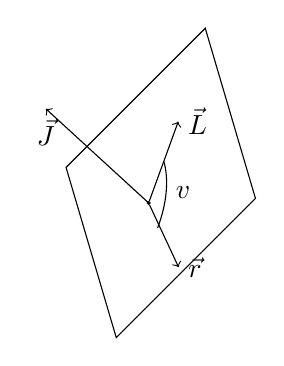
\begin{tikzpicture}[rotate around z=45, rotate around x=-45]
\draw (0,-0.3,0) -- (2.5,-0.3,0) -- (2.5,2.5,0) -- (0,2.5,0) -- cycle;
\draw[->] (1.,1.,0)node[draw,circle,inner sep=0] (o) {} -- (1.5,1.5,2)node[below] {$\vec{J}$};
\draw[->] (o) -- ++(295:0.9cm)node[right] {$\vec{r}$};
\draw[->] (o) -- ++(70:1.1cm)node[right] {$\vec{L}$}node [midway] (aux){};
\draw (aux) arc (0:-50:1) node[midway,right] {$v$};
\end{tikzpicture}

\label{fig:Lenztikz}

\end{figure}

\end{filecontents}


\begin{filecontents}{reducedproblem.tex}

%reduced problem

\begin{tikzpicture}

\node[circle,fill,inner sep=1pt,label=above:M] (M) at (0,0) {}; 
\draw (M)--++(30:1cm) node[circle,fill,inner sep=1pt,label=below:O] (O) {};
\draw[->] (O)--++(30:1.5cm) node[circle,fill,inner sep=1pt,label=above:m,yshift=1pt,xshift=1pt] (m) {} node[midway,above] {$\vec{r}$} ;

\node[circle,fill,inner sep=1pt,below=1cm of O,label=below:O] (O1) {}; 
\draw[->] (O1)--++(30:1.5cm) node[circle,fill,inner sep=1pt,label=above:m,yshift=1pt,xshift=1pt] (m1) {} node[midway,below] {$\vec{r_1}$} ;
\draw[->] (O1)--++(-150:1cm) node[circle,fill,inner sep=1pt,label=above:m,yshift=1pt,xshift=1pt] (m1) {} node[midway,below] {$\vec{r_2}$} ;
%\node (dida) at (7,0) {\parbox{8cm}{Siano m e M due masse puntiformi o a simmetria sferica: O \'e il centro di massa e $\vec{r}=\vec{r_1}-\vec{r_2}$ la distanza relativa.}};

\end{tikzpicture}

\end{filecontents}

\begin{filecontents}{ellipse.tex}

%ellisse

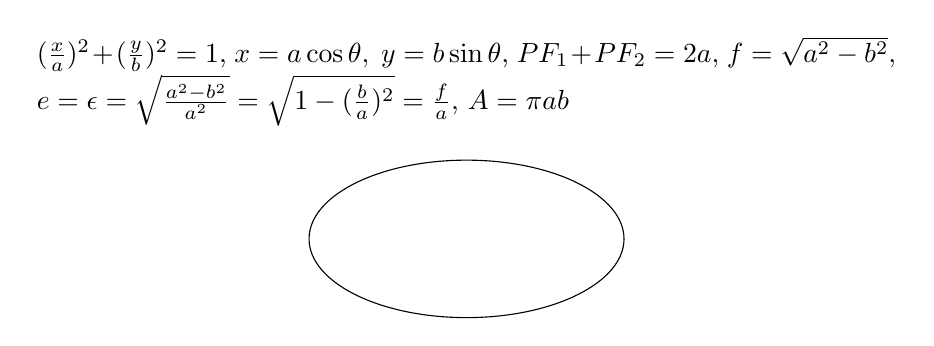
\begin{tikzpicture}

\draw ellipse (2cm and 1cm) node (o) {};
\node (prop) at (0,2) {\parbox{0.9\textwidth}{
$(\frac{x}{a})^2+(\frac{y}{b})^2=1$,
$x=a\cos{\theta},\ y=b\sin{\theta}$,
$PF_1+PF_2=2a$,
$f=\sqrt{a^2-b^2}$,
$e=\epsilon=\sqrt{\frac{a^2-b^2}{a^2}}=\sqrt{1-(\frac{b}{a})^2}=\frac{f}{a}$,
$A=\pi ab$}
};

\end{tikzpicture}

\end{filecontents}%%contain tikz files as filecontents

\addtobeamertemplate{block begin}{\setlength\abovedisplayskip{2pt}\setlength\belowdisplayskip{2pt}\setlength\abovedisplayshortskip{2pt}\setlength\belowdisplayshortskip{2pt}}

\addtobeamertemplate{block begin}{\vspace*{-3pt}}{}
\addtobeamertemplate{block end}{}{\vspace*{-3pt}}

\begin{frame}
  \titlepage
\end{frame}

% Section and subsections will appear in the presentation overview
% and table of contents.
%\frame{\tableofcontents[onlyparts]}

\begin{frame}[label={argomenti}]{Sistemi planetari: Sistema solare}
\tableofcontents[onlyparts]
\end{frame}

\begin{wordonframe}{Perch\'e studio queste cose?? Sviluppi; futuro.}
Osservazione sistemi planetari: luce emessa da stella/pianeta. Dischi protoplanetarii.
\end{wordonframe}

\part{Moti sistemi planetarii, struttura interna pianeti (emissione termica e non). Dischi di accrescimento.}\label{part:observables}
\section{Luminosit\'a di un pianeta.}

\begin{frame}{Luce riflessa e emissione termica}

\begin{block}{luminosit\'a monocromatica (emisfero illuminato)}
\begin{align*}
&L_{\lambda,P}=A_{\lambda}\Lambda_{\lambda,P}\\
&\Lambda_{\lambda,P}=\frac{L_{\lambda}^*\pi R_P^2}{4\pi r_{P*}^2}=0.25L_{\lambda}^*\frac{R_P^2}{r_{P*}^2}\\
&L_P=\int_{Vis.}A_{\lambda}\Lambda_{\lambda,P}=A\int_{Vis}\Lambda_{\lambda,P}\,d\lambda
\end{align*}
\end{block}
\begin{block}{Manitudine visuale}
\begin{align*}
&I_V=\int_{Vis}\frac{S_V(\lambda)D_{\lambda}(\theta) L_{\lambda,P}}{4\pi r_{P,T}^2}\,d\lambda\\
&m_V=-2.5\log{I_V}+\const{}
\end{align*}
Per un pianeta molto lontano dalla stella ($r_{T*}\ll r_{P*}$)
\begin{align*}
&m_V=m_{V_0}+10\log{r_{PT}}&\intertext{$m_{V_0}$ indipendente dalla distanza.}
\end{align*}
\end{block}
\end{frame}

\begin{wordonframe}{Albedo, emissione termica, magnitudine}
Un pianeta \'e caratterizzato da emissione nel visibile e nell'infrarosso: dell'energia radiante ricevuta da un'eventuale stella parte viene riflessa e parte assorbita e riemessa nell'infrarosso.

Un pianeta di raggio $R_P$ a distanza dalla stella $r_{P*}^2$ riceve $    \Lambda_{\lambda,P}=\frac{L_{\lambda}^*\pi R_P^2}{4\pi r_{P*}^2}=0.25L_{\lambda}^*\frac{R_P^2}{r_{P*}^2}$.

se riflette una percentuale $A_{\lambda}$ (albedo). quindi per un pianeta all'opposizione si ha
\begin{align*}
&I_V=\int_{Vis}\frac{S_V(\lambda)D_{\lambda}(\theta) L_{\lambda,P}}{4\pi r_{P,T}^2}\,d\lambda=\int_{Vis}\frac{S_V(\lambda)D_{\lambda}(\theta) A_{\lambda}L_{\lambda}^*R_P^2}{14\pi^2r_{P,T}^2r_{P*}^2}\,d\lambda\\
&m_V=-2.5\log{(\int S_V(\lambda)D_{\lambda}(\theta)A_{\lambda}L_{\lambda}^*\,d\lambda)}-5\log{R_P}+5\log{r_{PT}}+5\log{r_{P*}}+\const{}\\
&=-2.5\log{(\int S_V(\lambda)D_{\lambda}(\theta)A_{\lambda}L_{\lambda}^*\,d\lambda)}-5\log{(\sqrt{A'}R_P)}+5\log{r_{PT}}+5\log{r_{P*}}+\const{}
&r_{PT}=r_{P*}-r_{T*}
\end{align*}
\end{wordonframe}

\begin{frame}{Osservazione diretta: tecniche astrometriche}
Risoluzione del sistema in maniera visuale: la separazione angolare Sole/Giove sarebbe \SI{1}{\arcsec} gi\'a a \SI{5}{\parsec}.

Estrema differenza tra $L^*$ e $L_P$: per il sistema Sole/Giove nel visibile
\begin{align*}
    \frac{L_P}{L_*}=P(\lambda,\alpha)(\frac{R_P}{a})^2\approx\num{e-9}&\intertext{$P(\lambda,\alpha)$ dipende da albedo e fase a cui si trova il pianeta.}
\end{align*}

Effetto di selezione: pianeti lontani dalla stella ($a>\SI{10}{\astronomicalunit}$).
\end{frame}

\begin{wordonframe}{Orbita stellare}
Misura posizione e moti dei corpi celesti. The path of a star orbiting star-planet barycentre appears projected on the plane of the sky as an ellipse with angular semi-major axis $\alpha$
\begin{align*}
&a_*:a_{rel}=M_p:(M_p+M_*),\ a_{rel}=a_*+a_p
&\alpha=\frac{M_p}{M_*+M_p}a\approx\frac{M_p}{M_*}a\\
&\approx(\frac{M_p}{M_*})(\frac{a}{\SI{1}{\astronomicalunit}})(\frac{d}{\SI{1}{\parsec}})\expy{-1}\si{\arcsec}
\end{align*}
Angolo sotteso da semiasse maggiore orbita ellittica stellare attorno a cm:
\begin{equation*}
\theta=\frac{m_p}{r}(\frac{P}{M_*})\expy{3/2}
\end{equation*}
P(\si{\year}), masse in masse solari e r(\si{\parsec}).
\end{wordonframe}

\subsection{Orbita del pianeta}

\begin{frame}{Moto del pianeta}
Il moto di un singolo pianeta attorno ad una stella provoca un moto riflesso della stella attorno al centro di massa. Questo provoca perturbazione delle caratteristiche osservabili
\begin{itemize}
    \item Radial velocity
    \item angular (astrometric) position in the sky
    \item arrival time of periodic reference signal 
\end{itemize}
Il pianeta e la stella orbitano attorno al comune CM in orbite ellittiche chiuse con il CM come uno dei 2 fuochi.
\begin{align*}
&r=\frac{a(1-e^2)}{1+e\cos{\nu}}\\
&\frac{x^2}{a^2}+\frac{y^2}{b^2}=1\\
&b^2=a^2(1-e^2)
\end{align*}
\begin{figure}[!ht]
\centering
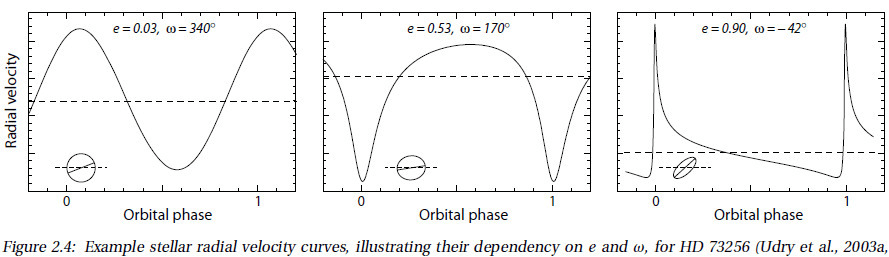
\includegraphics[width=(0.9\textwidth),height=\textheight,keepaspectratio]{vrcurve}
\caption{Stellar radial velocity curves: dependency on $e$ and $\omega$.}
\end{figure}
\end{frame}

\begin{wordonframe}{Moto del pianeta/stella attorno al CM}
Anomalia vera, $\nu(t), f(t)$: \'e l'angolo tra la direzione del pericentro e la posizione al tempo t misurata dal baricentro. L'anomalia eccentrica \'e l'angolo corrispondente all'anomalia vera riferito al cerchio ausiliario
\begin{align*}
&\cos{\nu(t)}=\frac{\cos{E(t)}-e}{1-e\cos{E(t)}}\\
&\tan{\frac{\nu(t)}{2}}=\sqrt{\frac{1+e}{1-e}}\tan{\frac{E(t)}{2}}
\end{align*}

L'anomalia medi \'e un'angolo relativo al moto medio attorno all'orbita: in un'orbita completa il pianeta non ha velocit\'a angolare costante ma una velocit\'a angolare media \'e specificata in termini del moto medio $n=\frac{2\pi}{P}$. L'anomalia media al tempo $t-t_p$ dopo il passaggio al pericentro \'e
\begin{align*}
&M(t)=\frac{2\pi}{P}(t-t_p)=n(t-t_p)\\
&M(t)=E(t)-e\sin{E(t)}
\end{align*}
\end{wordonframe}


\part{tecniche osservative}\label{part:tech}
\section{Photometry}

\begin{frame}{principal wide band photometric regimes}
\cite{mallama2017comprehensive}
\begin{itemize}
\item Johnson-Cousins system (Johnson et al. 1966, Cousins, 1976 and Cousins 1976)
\item Sloan system (Smith et al., 2002 and Fukugita et al., 1996)
\end{itemize}
\end{frame}



\section{Timing}

\begin{frame}{Moto della stella attorno al cm}
Se luce emessa dalla stella primari ha tempi caratteristici il moto ellittico dovuto alla presenza del pianeta produce variazioni nel cammino ottico della luce proporzionaleallo spostamento della primaria lungo la linea di vista
\begin{equation*}
    \tau_p=\frac{1}{c}\frac{a\sin{i}M_p}{M_*}
\end{equation*}
\end{frame}

\begin{frame}{Osservazioni di pulsar.}
Emettono segnale periodico regolare $\Pi\approx\si{\second}-\si{\milli\second}$. Il moto attorno al comune centro di massa Pulsar/pianeta causa una variazione del cammino ottico: il segnale arriva in anticipo o in ritardo.
Nel caso de lsistema Sole/Terra il sole percorre un'ellisse di semiasse maggiore circa $\frac{m_T}{\msun{}}a_T\approx\SI{500}{\kilo\meter}$: la differenza di cammino ottico causerebbe un $\Delta t\approx\SI{1}{\milli\second}$.
Sistemi non nati con la stella: formati in fase finale di evoluzione.
\end{frame}

\section{Microlensing gravitazionale.}

\begin{frame}{lente gravitazionale}
La presenza di materia (densit\'a di energia) distorce lo spazio-tempo e il la radiazione EM pu\'o essere deviata: la luce proveniente da un'oggetto lontano pu\'o essere deviata dal campo gravitazionale di un oggetto (lente) e quindi per l'oservatore risulta distorta e amplificata. 

\begin{definition}{Microlensing.}
Si parla di microlensing quando le immagini multiple dell'oggetto lontano non sono risolte.
\end{definition}
\end{frame}

\begin{frame}{Gravitational light bending}
\begin{figure}[!ht]
\centering
%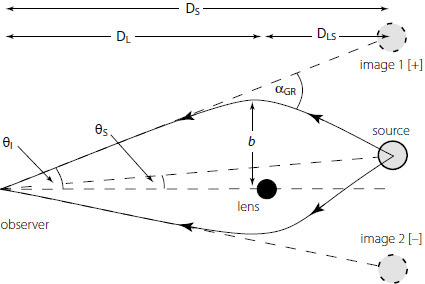
\includegraphics[width=(0.9\textwidth),height=\textheight,keepaspectratio]{lensing}
\caption{lensing.}
\end{figure}
\end{frame}

\begin{wordonframe}{Gravitational light bending}
\begin{definition}{Raggio di \sch{.}}
Il raggio di \sch{} \'e
\begin{equation*}
    R_S=\frac{2GM_L}{c^2}
\end{equation*}
\end{definition}
\begin{align*}
&\alpha_{GR}=\frac{4GM_L}{c^2b}=\frac{2R_S}{b}&\intertext{con la condizione che il parametro di impatto $b\gg R_S$}
\end{align*}
Lens equation:
\begin{equation*}
\theta_S=\theta_I-2R_S\frac{D_{LS}}{D_LD_S}\frac{1}{\theta_I}
\end{equation*}
\end{wordonframe}

\begin{frame}{Einstein radius.}
La sorgente lontana vedra la sua luminosit\'a amplificata dalla lente in proporzione all'Anello di Einstein
\begin{equation*}
    \theta_E^2=\frac{4GM_LD_{LS}}{c^2D_{OL}D_{OS}}
\end{equation*}
Le sorgenti galattiche possono essere stelle del nucleo galattico ($D_{OS}\approx\SI{10}{\kilo\parsec}$ e lenti tipic a met\'a strada).
Per $M_L\approx\msun{}$: $\theta_E\approx\si{\milli\arcsec}$.
Le dimensioni dell'anello di Einstein definiscono il livello di allineamento richiesto per avere una significativa amplificazione del segnale della sorgente.
Dimensioni lineari dell'anello di Einstein
\begin{align*}
    R_E=(1-y)\,d\theta=\sqrt{2y(1-y)R_Sd}
\end{align*}
con $d=D_{os}$, $yd=D_{LS}$, massime dimensioni lineari per $y=\frac{1}{2}$.
Il raggio di luce deve passare ad una distanza inferiore di $R_E$ dalla lente.
Inserendo quantit\'a tipiche per ricerca di esopianeti
\begin{align*}
&\theta_E\approx1.0(\frac{M_L}{\msun{}})\expy{\frac{1}{2}}(\frac{D_L}{\SI{8}{\kilo\parsec}})\expy{-\frac{1}{2}}(\frac{D_{LS}}{D_S})\expy{\frac{1}{2}}\si{\milli\arcsec}\\
&R_E\approx8.1(\frac{M_L}{\msun{}})\expy{\frac{1}{2}}(\frac{D_S}{\SI{8}{\kilo\parsec}})\expy{\frac{1}{2}}(\frac{D_LD_{LS}}{D_S^2})\expy{\frac{1}{2}}\si{\astronomicalunit}
\end{align*}
\end{frame}

\begin{frame}{Magnification}
\begin{figure}[!ht]
\centering
%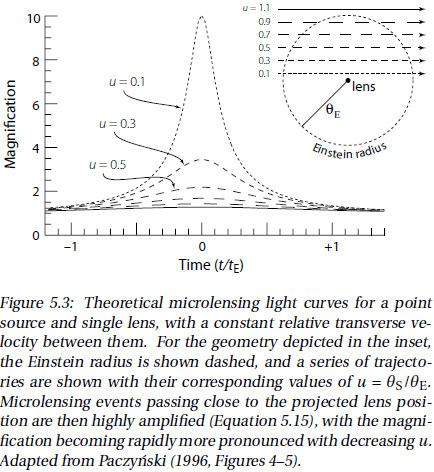
\includegraphics[width=(0.7\textwidth),height=\textheight,keepaspectratio]{lensinglcurves}
\caption{Microlensing magnification.}
\end{figure}
\end{frame}

\begin{frame}{Fatti}
\begin{itemize}
    \item In un cilindro di raggio $R_E$ e altezza $D_{OS}$ ho probabilit\'a $\frac{1}{100000}$ che ci sia una stella.
    \item Se la lente \'e costituita da pi\'u masse avremo una curva di luce con pi\'u picchi
    \item Nel caso di lente con sistema planetario la distribuzione dei picchi \'e detrminata dalla posizione dei pianeti: pi\'u efficace vicino all'anello di Einstein.
\end{itemize}
\begin{figure}[!ht]
\centering
%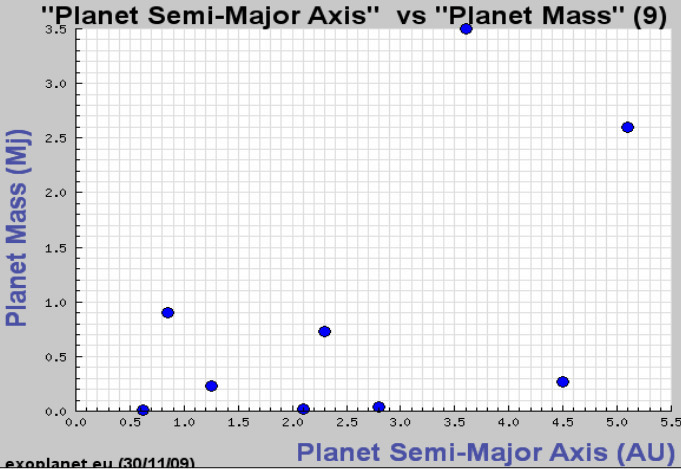
\includegraphics[width=(0.7\textwidth),height=\textheight,keepaspectratio]{mp-a-micro}
\caption{Massa pianeti vs semiasse per pianeti scoperti tramite microlensing.}
\end{figure}
\end{frame}

\section{Tecniche spettroscopiche (Misura velocit\'a radiale).}

\begin{frame}{Orbita stella attorno a CM}
\begin{figure}[!ht]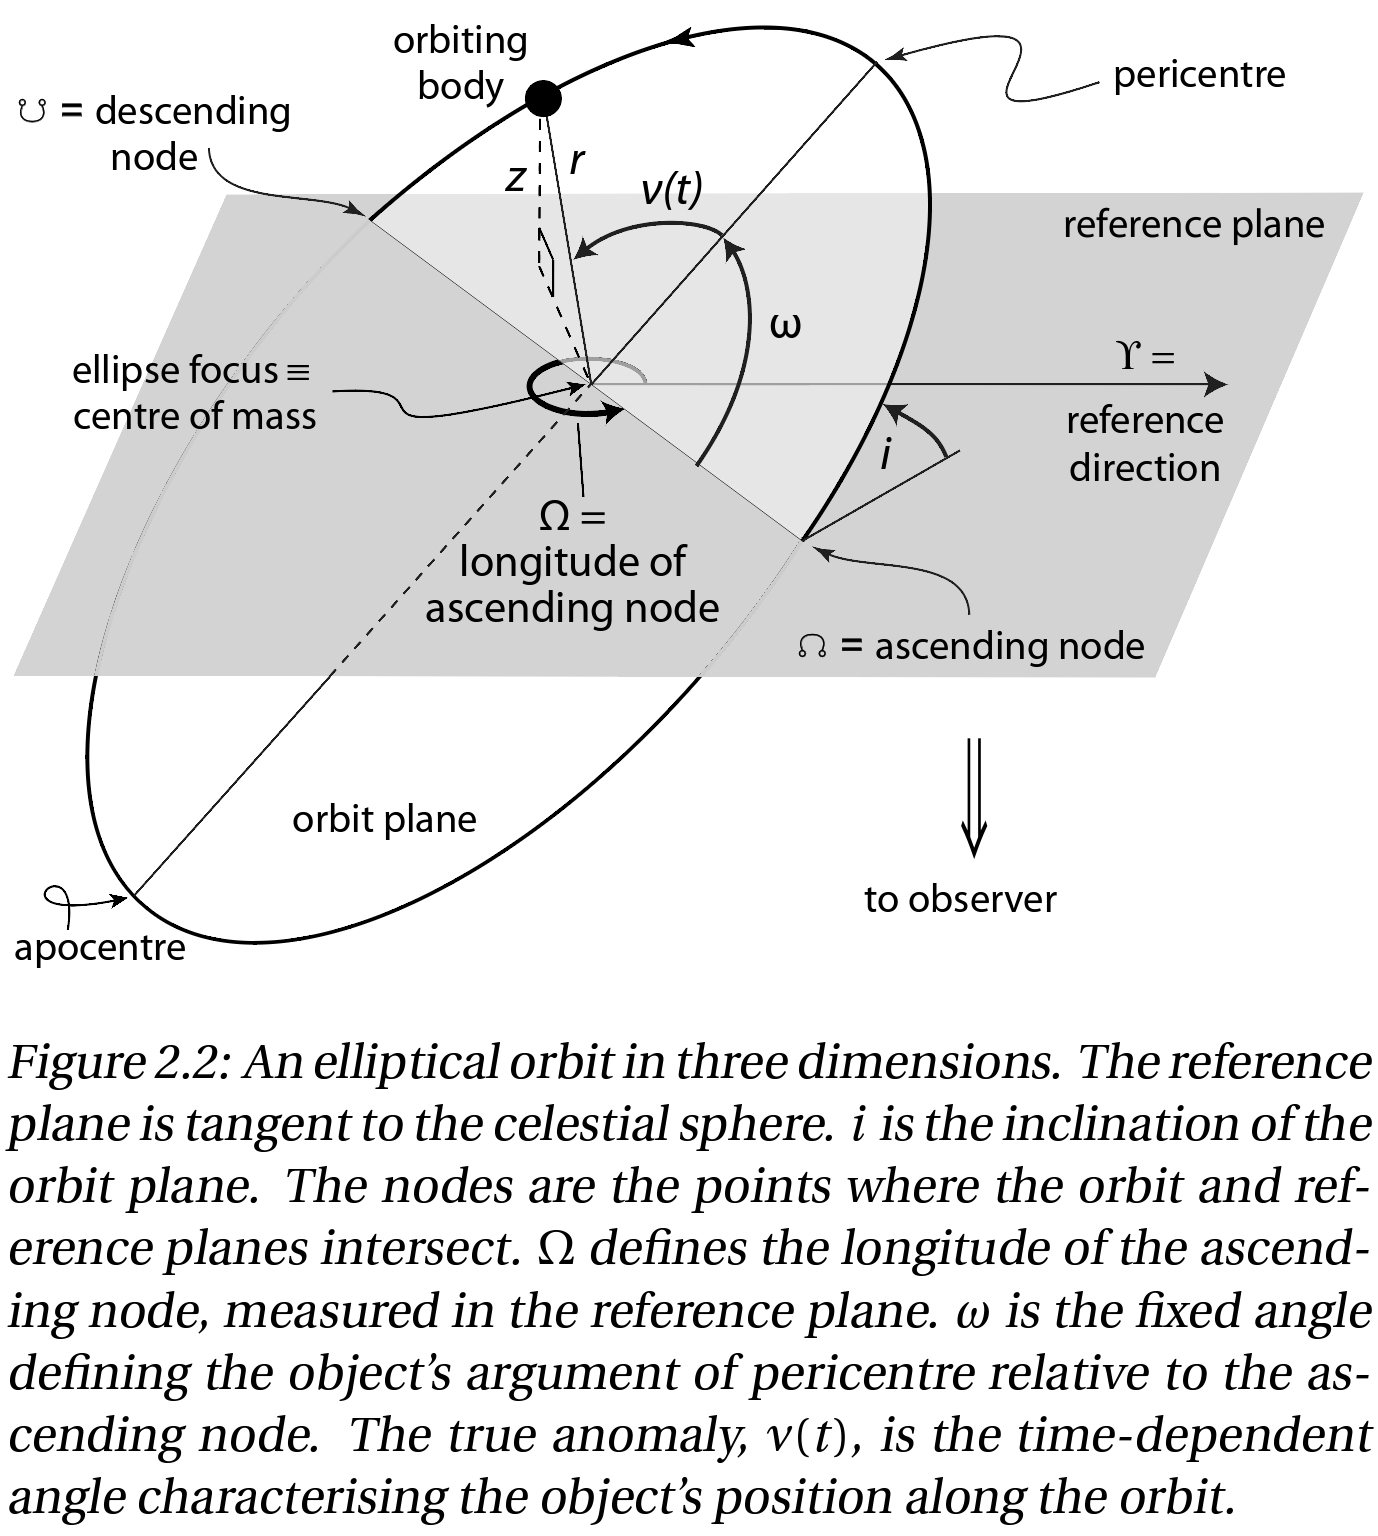
\includegraphics[trim={0cm 2cm 0 0},clip, keepaspectratio,height=0.5\textheight]{sightvelocity}\label{fig:sightvelocity}\end{figure}
\begin{align*}
&v_r=K[\cos{\omega+\nu}+e\cos{\omega}]\\
&K=\frac{2\pi}{P}\frac{a_*\sin{i}}{\sqrt{1-e^2}}\\
&K=\frac{2\pi}{P}\frac{a_*\sin{i}}{(1-e^2)\expy{1/2}}=(\frac{2\pi G}{P})\expy{1/3}\frac{M_p\sin{i}}{(M_p+M_*)\expy{2/3}}\frac{1}{(1-e^2)\expy{1/2}}
\end{align*}
\end{frame}

\begin{wordonframe}{Orbit specification}
\begin{columns}[T]\begin{column}{0.3\textwidth}
\begin{figure}[!ht]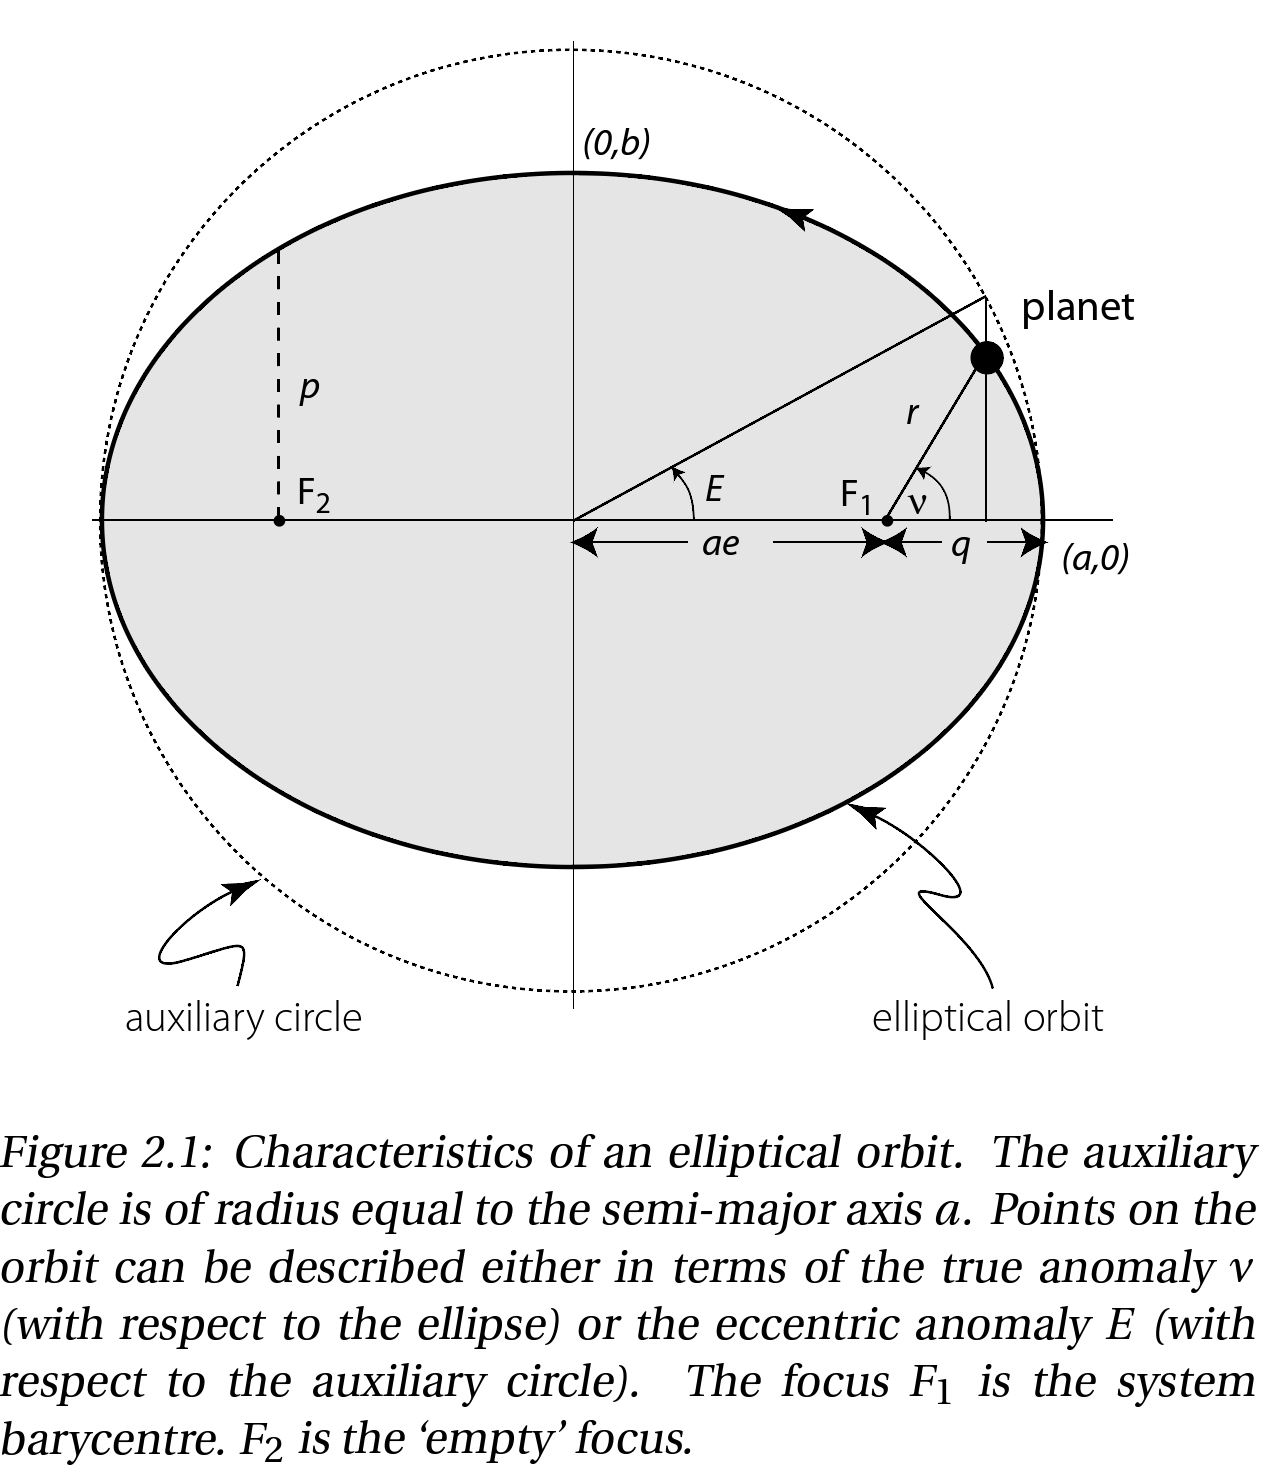
\includegraphics[trim={0cm 0cm 0 0},clip, keepaspectratio,width=0.99\textwidth]{ellipse}\label{fig:ellipse}\end{figure}
\end{column}\begin{column}{0.7\textwidth}
Ellipse: rel to focus $r=\frac{a(1-e^2)}{1+e\cos{\nu}}$, rel to center $\frac{x^2}{a^2}+\frac{y^2}{b^2}=1$.
\begin{align*}
&q=a(1-e)\\
&Q=a(1+e)\\
&p=a(1-e^2)
\end{align*}
$\nu(t)$ anomalia vera, $E(t)$ anomalia eccentrica, anomalia media $M(t)$, $t_p$ passaggio dal pericentro:
\begin{align*}
&\cos{\nu(t)}\frac{\cos{E(t)}-e}{1-e\cos{E(t)}}\\
&M(t)=\frac{2\pi}{P}(t-t_p)=n(t-t_p)
\end{align*}
\end{column}\end{columns}
\end{wordonframe}

\begin{wordonframe}{Variazione periodica velocit\'a radiale stella}
Variazione periodica della velocit\'a radiale dovuta al moto attorno al CM.
For the radial velocity semi-amplitude we have
\begin{align*}
&v_r=K[\cos{\omega+\nu}+e\cos{\omega}]\\
&K=\frac{2\pi}{T}\frac{A_*\sin{i}}{\sqrt{1-e^2}}\\
&K^2=\frac{G}{(1-e^2)}\frac{1}{a_*\sin{i}}\frac{M_p^3\sin^3{i}}{(M_*+M_p)^2}&\intertext{radial velocity measurement provide a value for mass function}\\
&\frac{M_p^3\sin^3{i}}{(M_*+M_p)^2}
\end{align*}
La terza legge di Keplero
\begin{equation}
(M^*+m_P)\sin^3{i}=\frac{4\pi^2a^3\sin^3{i}}{GP^2}
\end{equation}
$i$ \'e l'inclinazione dell'orbita rispetto al piano nella sfera celeste normale alla linea di vista.
\end{wordonframe}

\begin{frame}{Mass function}

Definisco la funzione delle masse
\begin{align*}
&f(M^*,m_P)=(M^*+m_P)\sin^3{i}\frac{m_P^3}{(M^*+m_P)^3}\\
&=\frac{4\pi^2}{GP^2}{a^*}^3\sin^3{i}\\
&f=\frac{PK_2^3}{2\pi G}&\intertext{$K_2$ is half the change in radial velocity.}\\
&f=\frac{M_1\sin^3{i}}{(1+q)^2}&\intertext{q \'e il rapporto tra le masse $M^*$ fratto massa oggetto non visibile $m_P$.}
\end{align*}
\end{frame}

\begin{wordonframe}{Radial velocity semi-amplitude}
Prendendo la coordinata z della stella lungo la linea di vista
\begin{align*}
&z=r(t)\sin{i}\sin{(\omega+\nu)}\\
&v_r=\dot{z}=K[\cos{(\omega+\nu)}+e\cos{\omega}]\\
&K=\frac{2\pi}{P}\frac{a_*\sin{i}}{(1-e^2)\expy{\frac{1}{2}}}
\end{align*}
Per il sistema Sole/Giove $K_k\approx\SI{12}{\meter\per\second}$ ($a=\SI{5.2}{\astronomicalunit}$, $P=\SI{11.9}{\year}$).
Sole/Terra $K_E\approx\SI{10}{\cm\per\second}$.
\end{wordonframe}

\begin{frame}{Keplerian observables}
\begin{columns}[T]\begin{column}{0.3\textwidth}
Descrizione orbita: $(a,e,P,t_p,i,\Omega,\omega)$.
\end{column} \begin{column}{0.7\textwidth}
\begin{figure}[!ht]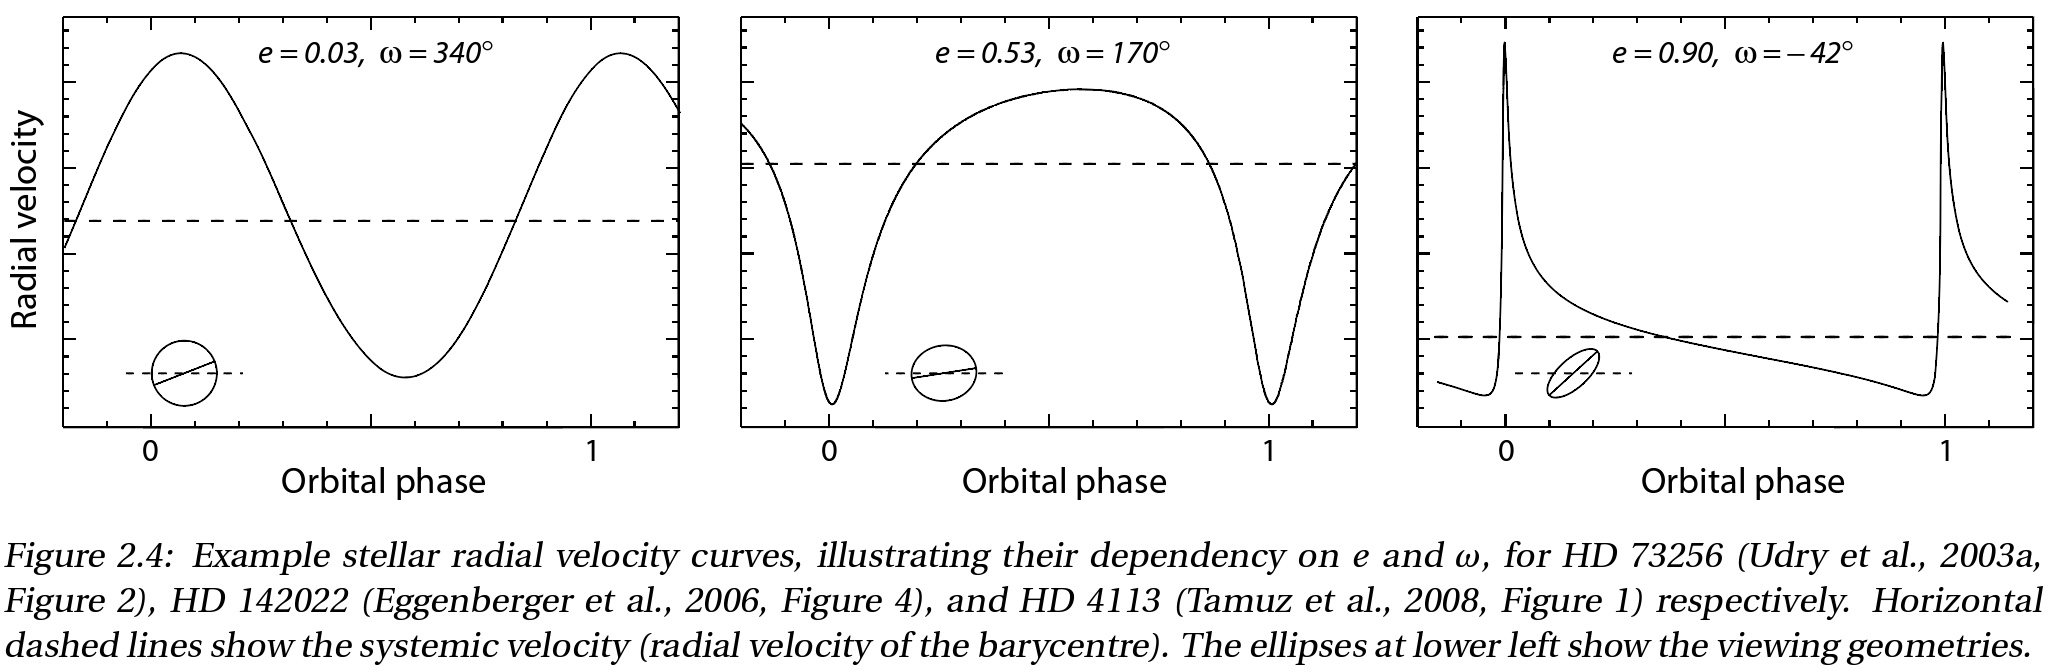
\includegraphics[trim={0cm 0cm 0 0},clip, keepaspectratio,width=0.9\textwidth]{orbitalphase.jpeg}\label{fig:orbitalphase}\end{figure}
\end{column}\end{columns}
\begin{align*}
&v_r=K[\cos{(\omega+\nu(t))}+e\cos{\omega}]+\gamma+d(t-t_o)
\end{align*}
con $K(a,e,m\sin{i},P)$: ottengo e, P, $t_p$, $\omega$, $m\sin{i}$.
\end{frame}

\section{Tecniche fotometriche: transiti.}

\begin{frame}{Transiti}
Abbiamo 4 osservabili
\begin{itemize}
    \item Il periodo P.
    \item La profondit\'a del transito $\Delta F$.
    \item Intervallo di tempo tra 1-4 $t_T$.
    \item Intervallo di tempo tra 2-3 $t_F$.
\end{itemize}
\begin{align*}
&\Delta F\approx(\frac{R_p}{R_*})^2\\
&t_T\approx13(\frac{M_*}{\msun{}})\expy{-\frac{1}{2}}(\frac{a}{\si{\astronomicalunit}})\expy{\frac{1}{2}}\frac{R_*}{\rsun{}}\si{\hour}
\end{align*}
La probabilit\'a che per un pianeta orientato arbitrariamente si possa osservare transito a eclisse secondaria \'e
\begin{equation*}
Pr\frac{R_*}{a}\approx0.005\frac{R_*}{\rsun{}}(\frac{a}{\si{\astronomicalunit}})\expy{-1}
\end{equation*}
data dall'area spazzata dall'ombra del pianeta sulla sfera celeste.
\end{frame}

\begin{wordonframe}{Probabilit\'a osservazione transito}
\begin{figure}[!ht]
\centering
%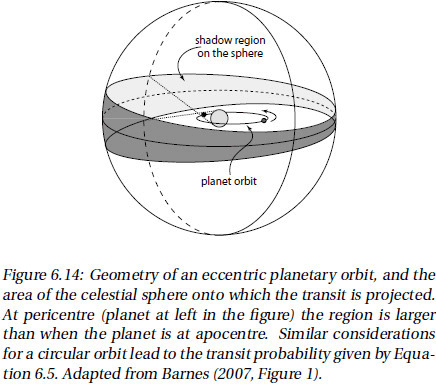
\includegraphics[width=(0.7\textwidth),height=\textheight,keepaspectratio]{sphereshadow}
\caption{Area della sfera celeste su cui \'e proiettato il transito.}
\end{figure}
\end{wordonframe}

\begin{wordonframe}{transito visto dalla terra}
\begin{figure}[!ht]
\centering
%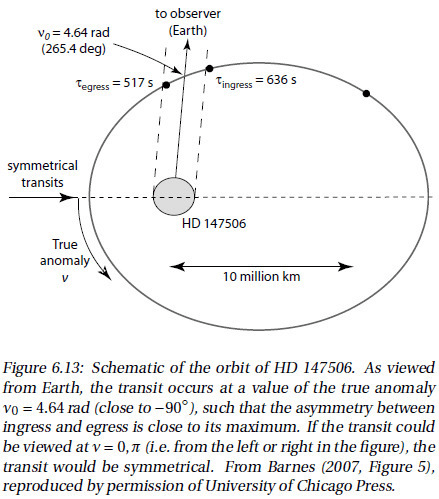
\includegraphics[width=(0.7\textwidth),height=\textheight,keepaspectratio]{transitex}
\caption{Transito visto dalla Terra.}
\end{figure}
\end{wordonframe}

\begin{wordonframe}{transiti: osservabili}
\begin{figure}[!ht]
\centering
%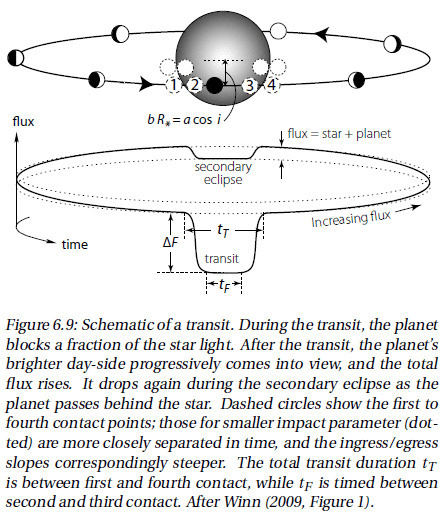
\includegraphics[width=(0.9\textwidth),height=\textheight,keepaspectratio]{transit}
\caption{Schematic of a transit and secondary eclipse (planet passes behind).}
\end{figure}
\end{wordonframe}

\begin{frame}{Fatti}
\begin{figure}[!ht]
\centering
%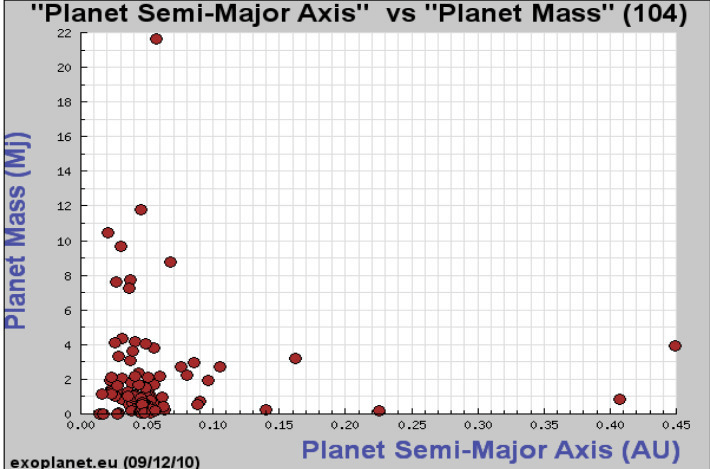
\includegraphics[height=0.9\textheight,keepaspectratio]{mp-atransit}
\caption{Massa pianeta vs semiasse per pianeti scoperti tramite transito.}
\end{figure}
\end{frame}

\begin{wordonframe}{Fatti}
\begin{itemize}
    \item Per un'eclissi totale Sole/Giove ho variazione $\Delta L\approx1\%$.
\end{itemize}
\end{wordonframe}


\end{document}